\documentclass{article}
\usepackage[utf8]{inputenc}
\usepackage[T1]{fontenc}
\usepackage[a4paper]{geometry}
\usepackage{amsmath}
\usepackage{amssymb}
\usepackage{graphicx}
\usepackage{rotating}
\usepackage{placeins}
\usepackage[slovak]{babel}
\usepackage{makeidx}
\usepackage[colorlinks=true,linkcolor=blue,urlcolor=black]{hyperref}
\usepackage{bookmark}

\renewcommand{\figurename}{Obr.}
\renewcommand{\tablename}{Tab.}
\newcommand{\overbar}[1]{\mkern 1.5mu\overline{\mkern-1.5mu#1\mkern-1.5mu}\mkern 1.5mu}

\makeindex


\begin{document}
	\title{Špecifikácia funkcionality Osciloskopu na semestrálny projekt z predmetu vnorené systémy}
	\author{Denis Vasko a Ján Urdianyk} 
	\maketitle
	\thispagestyle{empty}
	\newpage
	
	
	\tableofcontents
	\listoffigures
	\listoftables
	\newpage
	
\section{Funkcie osciloskopu}
\begin{itemize}
	\item Meracia mriežka (Graticule) 
	\item Ovládanie časovej základne - čas/horizontálny diel
	\item Vertikálne škálovanie - škálovanie konštantou, zmena polarity
	\item X-Y mód (vykreslenie závislosti napätia na kanále Y od napätia na kanále X)
	\item Horizontálne škálovanie - pre X-kanál v X-Y móde
	\item Vertikálny posun - pre oba kanály zvlášť
	\item Horizontálny posun - pre oba kanály zvlášť
	\item Možnosť zobrazenia časového priebehu napätí na oboch kanáloch zároveň (Prepínanie len Y, len X, oba X aj Y alebo X-Y mód)
	\item Tigrovaný vstup - štart zobrazenia pri dosiahnutí dostatočnej úrovne napätia na sledovanom/ných kanáloch
	\item Hold-off - po trigrovaní vstupu sa ďalšie vykreslenie nemôže uskutočniť kým neprejde daný čas - cooldown trigrovania
	\item Automatické prekresľovanie - aj keď napätie na kanály nedosiahne dostatočnú hodnotu na trigoravnie, aj tak sa periodicky kanál prekresľuje s istou periódou. V prípade, že napätie na kanály dosiahne trigrovacie napätie, automatické prekresľovanie sa vypne (restne sa časovač), potom sa znovu zapne po neprítomnosti trigrovacieho napätia na kanály
	\item Jednorázové vykreslenie - vykreslenie jedného merania 
	\begin{itemize}
		\item štart pri presiahnutí úrovne napätia
		\item štart po istom čase 
	\end{itemize}
\end{itemize} 
\section{Vstupný delič napätia}
Podľa potreby by sme na vstup pripojili delič napätia s dostatočne veľkými odpormi pre určené napätie. Zenerová dióda tam nemusí byť, napätie na MCU by boli napätie medzi svorkami C,D pričom vstupné napätie by sa privádzalo na svorky A,B.

\begin{figure}[!h]
	\centering
	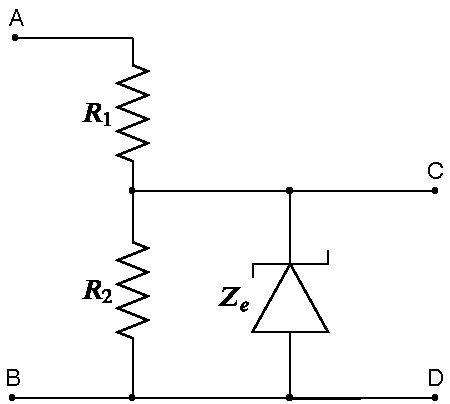
\includegraphics[width=0.4\linewidth]{../Obrazky/inputdivider.pdf}
\end{figure}
	
	
	%\printindex
\end{document}
